\documentclass[12pt]{article}

%Page Formatting
\usepackage[margin=1in]{geometry} 
 \usepackage{fancyhdr} 
\setlength{\headheight}{14.5pt}
\pagestyle{fancy}
\usepackage{lastpage}

%Math Formatting
\usepackage{amsmath,amsthm,amssymb}
\usepackage{siunitx} \sisetup{per-mode=fraction}
\usepackage{blkarray}
\usepackage{breqn}

%Section Formatting
\usepackage{etoolbox}
\usepackage{sectsty}
\sectionfont{\fontsize{16}{16}\selectfont}
\subsectionfont{\fontsize{14}{15}\selectfont}
\apptocmd{\thebibliography}{\raggedright}{}{}
\usepackage[title]{appendix}

%Paragraph Formatting
\edef\restoreparindent{\parindent=\the\parindent\relax}
\usepackage{parskip}
\restoreparindent
\newcommand{\just}{\textbf{Justification: }}
\newcommand{\expl}{\textbf{Explanation: }}

%TOC Formatting
\usepackage{url}
\usepackage[linkcolor=black,bookmarksopen=true]{hyperref}
\usepackage{bookmark}

%Table/Figure Formatting
\usepackage{graphicx}
\usepackage{booktabs}
\usepackage{caption} 
\captionsetup[table]{skip=10pt}

%Code Formatting
\usepackage{listings}
\usepackage{color} %red, green, blue, yellow, cyan, magenta, black, white
\definecolor{mygreen}{RGB}{28,172,0} % color values Red, Green, Blue
\definecolor{mylilas}{RGB}{170,55,241}
\lstset{language=Matlab,%
    %basicstyle=\color{red},
    breaklines=true,%
    morekeywords={matlab2tikz},
    keywordstyle=\color{blue},%
    morekeywords=[2]{1}, keywordstyle=[2]{\color{black}},
    identifierstyle=\color{black},%
    stringstyle=\color{mylilas},
    commentstyle=\color{mygreen},%
    showstringspaces=false,%without this there will be a symbol in the places where there is a space
    numbers=left,%
    numberstyle={\tiny \color{black}},% size of the numbers
    numbersep=9pt, % this defines how far the numbers are from the text
    emph=[1]{for,end,break},emphstyle=[1]\color{red}, %some words to emphasise
    %emph=[2]{word1,word2}, emphstyle=[2]{style},    
}

\begin{document}

\lhead{Team \#11762}
\rhead{Page \thepage{} of \pageref{bibliography}}

\section*{Executive Summary}
\addcontentsline{toc}{section}{Executive Summary}
As a result of excessive prescriptions and a history of substance abuse, the United States has today found itself in the midst of an opiod addiction crisis. The U.S. government has throughout the past decades recognized the ramifications of drugs on health and society at large and instituted regulations on the use of such substances. However, these substances have continued to be abused by many. Over the course of analyzing the drug crisis, we created models to predict the scale, causes, and costs of drug addiction in our society.

In recent years, the consumption of e-cigarette and vape products has skyrocketed, especially among adolescent Americans. To better understand the scale of this consumption and its effect on nicotine consumption (assuming no policy changes to combat usage), we created a logistic growth model to predict the proportion of teenagers who used nicotine-based vape products over the next decade. Based on the model we fit, we concluded that 36.18\% of teenagers in the year 2029 would use vape products, or approximately 6.1 million teens. Additionally, we modeled the growth of the adult vaping population by adding the portion of teens coming of age who vaped to the existing number of vaping adults, finding that 23.6 million adults would be using vape products in the year 2029, amounting to a total of 29.7 million total vape users in that year.

While it is impossible to definitively predict substance abuse by any person, there exist metrics documented by government and nonprofit organizations such as the Substance Abuse and Mental Health Services Administration (SAMHSA), which detail percentages of demographics that engage in drug-related activities. This information, within which exist striking trends, served a central role in our solution. We calculated weight values, ratios between a group’s measure and the average measure of all groups. Combining these weight values of all the measures into a product gives a measure of how likely a person is to become addicted. We used this approach to test ten people with randomly assigned characteristics (e.g. income, residence population density) for their tendency to become addicted to the following: marijuana, nicotine, alcohol, and opioids. We found that at our hypothetical high school of 300 students, there would be 6 opiate users, 26 marijuana users, 162 nicotine users, and 34 alcohol users.


To determine a metric to rank nicotine, opioid, marijuana, and alcohol based on their ramifications to financial and non-financial matters, we quantified factors of medical cost, employment, drug costs, and life expectancies into U.S. dollars. We made per capita values in dollars for the cost of being addicted to each drug  and  determined that marijuana is the least harmful drug, followed by nicotine, alcohol, and opioid at the worst.


\newpage
\tableofcontents

\section{Introduction}

\subsection{Background}
Drug abuse has contributed to growing issues in the United States such as automobile accidents, violence, child abuse, crime, unemployment, and homelessness. Drugs alter brain function and in cases such as driving, this altercation can impair the driver’s ability to make the appropriately rapid decisions necessary to be a safe driver. In 2010, a study revealed that 11\% of crashes that resulted in a death involved a driver that was under the influence of a drug \cite{three}. Addictions to substances such as alcohol, nicotine, marijuana, and opioids also impact the quality of life of an individual through health and financial factors. Substance abuse impacts over 23.6 million Americans \cite{one} and nationally costs more than \$200 billion in healthcare \cite{two} and \$540 billion in other expenses due to crimes and lost productivity \cite{two}. With the recent opioid crisis, 2.1 million people have been reported to have an opioid use disorder in 2017 with overdosing accounting for 47,600 deaths \cite{four}.

The impact of substance abuse has ramification that extend to society and therefore the race to curb substance abuse has escalated. Regulations from the FDA have increased on drugs as well as products that acts as vessels, like vape pens; however, as regulations increase so does opposition. As more research is done about the impacts of drugs, it becomes increasingly imperative to determine methods of regulation based on personal health risks presented as well as societal impacts. 


\subsection{Restatement of Problem}
In order to address the growing addiction to substances such as tobacco, alcohol, and narcotics, we were tasked to create solutions for the following problems:
\begin{itemize}
    \item Generate a model to predict the impact of vaping on new usage of nicotine over the next 10 years and compare this trend to past cigarette trends. 
    
    \item Generate a model that considers internal and external factors and use the model to simulate the likelihood that a given individual will use a given substance. Then use the model produced to predict how many students of 300 seniors are likely to use the following substances:
    \begin{itemize}
        \item Nicotine
        \item Marijuana
        \item Alcohol
        \item Unprescribed Opioids
    \end{itemize}

    \item Develop a comprehensive metric for the impact of substance use taking into consideration financial and non-financial factors and rank the substances listed above in terms of the severity of their impact.
\end{itemize}

\section{Darth Vapor - The Spread of Vaping}
\subsection{Defining Variables}
\begin{itemize}
\item \textbf{Input:} Years

\expl We track the percentage of teen vape usage over time in years.

\item \textbf{Output:} Proportion of teens who vape

\expl Through our logistic model, we mathematically predict the proportion of American teens who vape in a specific year, t.

\item \textbf{Output:} Number of teens who vape

\expl We multiply our model’s prediction of the proportion of teen vape usage for a specific year, t, by the population of total teens in the United States to calculate the population of teens who vape.

\item \textbf{Output:} Number of adults who vape

\expl We add the number of existing adults who use vape products to the sum of teens using vape products that transition into adulthood starting from a specific year, t0 , to calculate the total population of adults that vape.

\item \textbf{Output:} Total number of Americans who vape

\expl We find the sum of the number of teens who vape and the number of adults who vape to determine the total number of Americans that vape.

\end{itemize}

\subsection{Assumptions}
In order to simplify the model and calculations, the following assumptions were made:
\begin{enumerate}

\item People who switch to vaping from cigarettes do not contribute to additional nicotine consumption.

\just Predictions are to be made in relation to the spread of nicotine usage due to vaping. For those who smoked in the past and later transitioned to vaping, the nicotine usage for these individuals remains the same – simply their method of intaking the substance has altered.  

\item Teens\footnote{We use ``teens'' herein to refer only to those aged 14-18 (i.e. high school aged adolescents).} who vape did not smoke before.

\just In order to simplify the calculation of how vaping impacts nicotine usage, we assumed that all teens were not previously exposed to cigarette usage and teens who vape are considered newly introduced to nicotine use. 

\item Teen vape usage is equivalent to the average of vape usage among 10th and 12th graders.

\just The assumption made is that the average of data from 10th graders and 12th graders provides a fair average for high school usage. Data provided includes the statistics for 8th, 10th, and 12th graders, thus giving enough of a trend for high school vaping. Also considering the missing 9th and 11th grade data, it simplifies the process to use the 10th and 12th grade data provided to draw necessary trends.

\item E-cigarette statistics are analogous to vaping statistics. 

\just Starting in the years 2015-2018, we used Monitoring the Future data for vaping tobacco because in both data sets included 2015 in which the usage of e-cigarettes and vaping were very close which implies that the title “E-cigarettes” versus “vaping” are interchangeable. 

\item Teen vape trends will level off at a carrying capacity similar to teen cigarettes trends from the the past, 36.4\%.

\just In order to create a model of trends in vaping among teens, it is necessary to determine a trend line that would potentially fit the data. Using the given data on teen cigarettes and realizing that the usage reaches a carrying capacity, it can be stipulated that teen vape usage will follow a similar trend. 

\item The only growth of the proportion of adults who vape will come via teen vape users becoming

\just Though there is presumably some amount of existing adults who take up vaping nicotine, historical data of adult e-cigarette/vaping usage was not forthcoming beyond the most recent year of data. As a result, we could not model this kind of growth accurately. Since vaping is predominantly a youth phenomenon anyway, we opted to assume that only adults who took up vaping as teenagers would add to the existing population of adult vape users.

\item The 14-18 year old population will remain relatively constant at 16.77 million teens in the US. 4.21 million Americans enter adulthood every year.

\just In order to model predictions of nicotine spread among teens, a trend in teen population must be established. According to the Department of Health and Human Services, the teen population will remain relatively constant over the next several decades \cite{hhsPopulation}. We then calculated that their approximately 16.77 million high school age children currently in the United States \cite{numberOfTeens}. 

\item No policy initiatives will be undertaken to reduce the proportion of teens who vape.

\just Though this is not true as many organizations, including several levels of government, are planning to undertake efforts to reduce teenage vaping, we found that predicting the effects or even existence of such efforts would be arbitrary in nature. We thus chose to predict the proportion assuming the status quo holds. We feel that this assumption makes our model less arbitrary and in fact helps it to serve as a useful guide to policy makers in determining the success of certain initiatives compared to taking no action at all. 
\end{enumerate}

\subsection{Development of the Model}
The below steps summarize the approach we took to modeling this problem:
\begin{enumerate}
    \item We first model the growth of the proportion of teens who use nicotine through vaping over time
    \item We then multiply the proportion of teens who vape by the total number of teens in the United States (which we assumed to be constant at 16.77 million) to calculate the total number of teens who vaped nicotine/tobacco.
    \item Next, we calculate the existing number of adults who vape in the United States based on the proportions provided to us. 
    \item To calculate the growth of the adult vaping population, we multiply the number of teens entering adulthood by the proportion of teens that year who use vape products. We add this figure to the existing vaping adult population to calculate the new total adult vaping population.
\end{enumerate}

\subsubsection{Teenage Proportion Growth}
As the population of greatest concern, we first modeled the growth of teenage nicotine consumption through vaping. We chose to model the proportion of teens who vape as a logistic growth model\footnote{The data that the model was fit to was obtained from two combined sources: the 2016 Surgeon General's report regarding e-cigarette use among young adults \cite{cdcTeenVaping} and the annual Monitoring the Future survey \cite{mtfData}. We did so as they covered different periods of time and showed similar statistics in their overlapping proportions, giving us confidence that we could safely combine them.}.

We chose logistic growth because it effectively fits the characteristics of the real-life situation: it begins with a slow period of growth, followed by a period of very quick growth, and finally, a slowing of growth as the proportion reaches some carrying capacity. The growth of e-cigarettes and vape products similarly began slowly as the products gained traction and then underwent a sustained period of quick growth among teenagers. Of course, as there is a finite proportion of teens willing to vape under any circumstances, the growth would eventually slow drastically as that upper limit was approached.

We fit our logistic model \cite{logReg} with a carrying capacity of the proportion $p_{v,T} = 0.364$ or 36.4\%, where $p_{v,T}$ is the proportion of teens at some given time who vape regularly. We chose this (see Assumption 5) as this was the proportion of teens who consumed cigarettes at its peak and therefore served as a non-arbitrary upper limit to the proportion of teens who would vape regularly.

\begin{figure}
    \centering
    \includegraphics[width=\textwidth]{"Teen Vape Usage Graph"}
    \caption{A graph showing the predicted proportion of teens who use vape products over time. The red line denotes the logistic growth model created for prediction purposes.}
    \label{fig:predTeenProp}
\end{figure}

Figure \ref{fig:predTeenProp} shows the logistic growth model created to predict the proportion of teens who will use vape products in some given year. The logistic growth function can be defined as:
\begin{equation}
    p_{v,T}(t)=\frac{36.4}{1+e^{-0.42179\left(t-2016.933\right)}}
\end{equation}
\noindent where $p_{v,T}$ is the proportion of teens who vape in some year $t$.

\subsubsection{Adult Vaping Population Growth}
In order to accurately capture the use of vape products of the whole population, we must also consider adult usage of the products. We were not able to find historical data of e-cigarette or vape product usage for adults other than for the most recent year, so we chose to assume that the only addition to the adult vaping population would come from teens entering adulthood (see Assumption 6). 

As such, the total number of adults using vape products can be calculated by adding the existing number of adult users to the sum of teens using vape products that have entered adulthood since the starting year. In 2017, the CDC reported that the proportion of adults in the United States who use e-cigarettes was 2.8\%, or 6.93 million people \cite{cdcAdultTobacco}, and, as established in Assumption 7, 4.11 million teens enter adulthood annually. Thus, the total number of adults who use vape products can be modeled as

\begin{equation}
    P_{v,A}(t) = 6.93 + \sum_{t_0=2017}^{t} 4.11 \times \frac{36.4}{1+e^{-0.42179\left(t-2016.933\right)}}
\end{equation}

\noindent where $P_{v,A}(t)$ is the predicted number of adults (in millions) who vape in some given year $t$.

\subsubsection{Combining Teen and Adult Models}
To obtain the total number of Americans who use nicotine through vape products, we can combine Equations 1 and 2 as such:

\begin{equation}
    P_{v,USA}(t) = 16.77 \times \frac{36.4}{1+e^{-0.42179\left(t-2016.933\right)}} + 6.93 + \sum_{t_0=2017}^{t} 4.11 \times \frac{36.4}{1+e^{-0.42179\left(t-2016.933\right)}}
\end{equation}

\noindent where $P_{v,USA}(t)$ is the total number of Americans who use vape products regularly in millions.

\subsection{Results of the Model}

\begin{table}[]

\begin{tabular}{@{}lll@{}}
\toprule
Years & Predicted \% & Actual \% \\ \midrule
2013  & 5.821        & 4.5       \\
2017  & 18.46        & 14.85     \\
2021  & 30.85        & -         \\
2025  & 35.23        & -         \\
2029  & 36.18        & -         \\ \bottomrule
\end{tabular}
\quad
\begin{tabular}{@{}lll@{}}
\toprule
Years & Predicted & Actual   \\ \midrule
2013  & 0.9761    & 0.75465  \\
2017  & 3.095     & 2.490345 \\
2021  & 5.174     & -        \\
2025  & 5.908     & -        \\
2029  & 6.067     & -        \\ \bottomrule
\end{tabular}
\caption{The first table shows predicted proportion vs actual proportion of teens using vaping products for the given years. The second table gives the predicted vs actual number of teens using vaping products in millions of people.}
\label{table:teenUsage}
\end{table}

Table \ref{table:teenUsage} shows the predicted and (when present) the actual proportion and number of teens who use vape products in various years based on Equation 1. Table 2 shows the predicted number of adults and Americans as a whole who use vaping products for the given years.

We then conclude based on our models that 10 years from now (2029), 36.18\% of American teenagers, or 6.067 million teenagers, would be using vaping products (assuming no intervention in the current trends, of course). Additionally, we conclude that 23.61 million American adults would be using vape products, amounting to a total of 29.67 million Americans vaping in the year 2029.

\begin{table}[]
\begin{tabular}{@{}lll@{}}
\toprule
Years & Adults & All   \\ \midrule
2017  & 7.689  & 10.78 \\
2021  & 12.1   & 17.27 \\
2025  & 17.7   & 23.61 \\
2029  & 23.61  & 29.67 \\ \bottomrule
\end{tabular}
\caption{The predicted number of adults and predicted number of all Americans who use vape products in millions of people for the given years. Calculated using Equation 2 and 3.}
\end{table}

\subsection{Model Assessment and Analysis}
\subsubsection{Strengths}
\begin{itemize}
    \item Our logistic model accurately reflects the pattern of growth that would take place in the proportion of teens who vape. 
    
    \expl Because there is a limited population and because there will always be a portion of that population that will not intake a substance, it logically follows that a trend line for a substance like nicotine will eventually level out at an effective maximum after a period of growth.
    
    \item The model does not make any arbitrary assumptions about turning points/extrema or the undertaking of attempts to reduce nicotine consumption in the trend line.
    
    \expl The model does not depict any attempt made by outside forces to reduce the use of vape products in the general population. This is a strength because it avoids arbitrary conclusions and serves as a useful guide for policy makers to analyze a scenario in which no action is taken and from there conclude what actions are necessary and effective.

\end{itemize}

\subsubsection{Weaknesses}
\begin{itemize}
    \item We assume a potentially incorrect "carrying capacity" upper limit for our logistic growth matter.
    
    \expl Because the trend line predicts future values, it follows that there is no way to know the carrying capacity of vaping until it is potentially reached. Thus, we used the maximum proportion of teen cigarette use as a guideline of what the carrying capacity for vaping might be in the future. 
    
    \item Possible growth for adult nicotine usage due to existing adults beginning to vape is not factored in to the prediction models. 
    
    \expl Any increase in vaping in adult populations is attributed to teens who vape and become adults once they turn 18. The current number of adults who vape is included in our model, but no additional growth from solely adult populations is included as we could not find enough data to predict it accurately. With this data, we could easily implement this into our model, however.
\end{itemize}

\subsubsection{Sensitivity Analysis}
We created three related models in this part. The first one was the logistic growth model for the proportion of teens who would use vape products in a given year. Given the small amount of data that the model was trained on, it would be fairly variable if the inputs were changed slightly. However, given the defined carrying capacity value and the relatively strong fit ($RMSE=3.01$), the model fits the data fairly strongly. 

The second two models were the ones predicting the number of adults and Americans as a whole using vape products. Because these models are both dependent on a summation of the first model, they are largely more sensitive and thus minor variations in the data that the initial logistic model was trained on could have a great impact on the number of people that these models compute.

\subsubsection{Comparison to Cigarettes}
Both the trends in the percentage of teens who vape and the adult per capita cigarette consumption have trends of rapid growth in usage when first introduced. Both vape and cigarettes contain nicotine and thus consumption of both products would logically have similar trends in the increase of usage at their introduction. In the graph of adult per capita cigarette consumption (see Figure \ref{fig:cigGrowth}), the rapid growth is followed by a trend of decreasing consumption. It can be presumed that this decrease is a result of research and publications about the consequences to health due to smoking and increasing regulations on cigarettes. 

In our model of the percentage of teens who vape, the trend shows that consumption increases until it reaches a carrying capacity, but never decreases. The model does not show any decrease because it does not attempt to predict the effect of future research on health concerns or possible regulations on vaping. Instead, our model serves as a prediction for the trend that vaping will follow if no such regulation is put into place and therefore acts as a precaution for regulation agencies on the future of vaping should it go unchecked. 

\begin{figure}
    \centering
    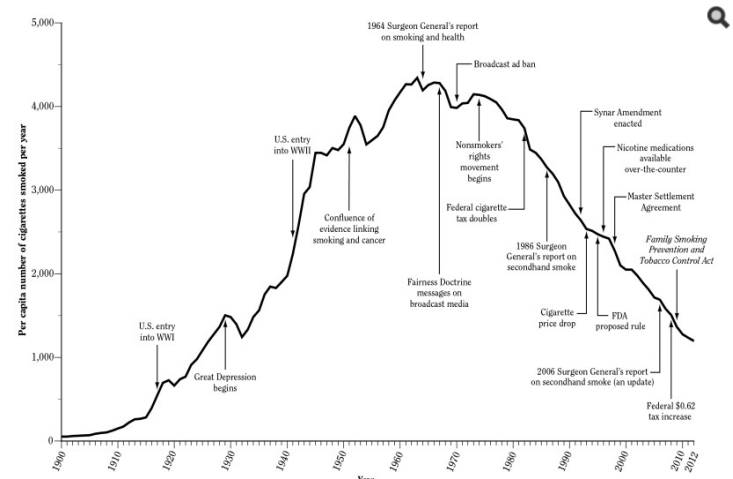
\includegraphics[width=14cm]{historicalcigarette}
    \caption{A graph of cigarette consumption in the United States since 1900 \cite{cdcTeenVaping}. Note the rapid rise in cigarette consumption that is analogous to the fast growth portion of our logistic model.}
    \label{fig:cigGrowth}
\end{figure}

\section{Above or Under the Influence? - Probability of Drug Use}

\subsection{Defining Variables}
\begin{itemize}
    \item \textbf{Input:} Income 
    
    \expl The income bracket of the individual based off of the poverty line (20k). The brackets we use are as follows: 
    \subitem Less than \$20,000 
    \subitem \$20,000 - \$40,000 
    \subitem More than \$40,000
    
    Because income correlates to substance abuse (inversely, most often), we found it to be a strong predictor of use of certain drugs.
    \item \textbf{Input:} Race
    
    \expl The race of the individual. The four categories of races considered for our model are White, Black, Hispanic, and Asian. We include race to serve as a crude indicator of genetic predispositions to substance abuse across humankind.
    
    \item \textbf{Input:} Gender 
    
    \expl The gender of the individual (male or female).
    
    \item \textbf{Input:} Urbanization/population density of location 
    
    \expl The density of population (urbanization) of the residence for the individual. We grouped this variable into the following three categories: 
    \subitem Urban - large metro (50,000 or more people)
    \subitem Suburban (urban clusters) - small metro (2,500 - 50,000 people)
    \subitem Rural - rural nonmetro  (less than 2,500 people)
    
    Definitions courtesy of the Census Bureau \cite{censusDesignation}. 
    
    \item \textbf{Input:} Substance
    
    \item The substance that we are determining the probability of usage for. The four drug categories we are analyzing in this section are nicotine, marijuana, alcohol, and unprescribed opiates.
    
    \item \textbf{Output:} Probability that a given person with traits will use a specific substance.
    
    \expl We will additionally determine the predicted number of people in a diverse high school who would use specific substances. 

\end{itemize}

\subsection{Assumptions}
\begin{itemize}
    \item “Use” means used the substance at least once a month.
    
    \just For the simplicity of creating a model that can predict use of a substance there needs to be an assumption made on the definition of “using” a substance. For the purposes of the question we have assumed that to be considered “use” of a substance, the individual users it at least once a month. As a result of this assumption, we opted to use Monitoring the Future's data of drug use at least once a month \cite{mtfData}
    
    \item The national average proportion of users of a certain drug can be used as a baseline probability that a given person would use it. 
    
    \just In order to predict the probability that someone would use a substance and determine the number of people within a demographic that would use a substance, a baseline must be established. From this baseline, we will make adjustments based on a person's specific traits to determine their true probability of using a certain substance.
    
    \item The input variables are not correlated with each other.
    
    \just Though this is not true (e.g. race \textit{is} correlated with income) in real life, it is impossible for us to quantify the exact amount of correlation and factor it out of our predicted probabilities. We therefore assume that it does not exist, leading to over/underestimation in some cases.
\end{itemize}

\subsection{Development of the Model}
We took a weighted probability approach to this problem. First, we compiled data regarding the proportion of people with different traits (e.g. race, gender, etc.) who use the substances in question from the extensive 2016 National Survey on Drug Use and Health conducted by the Substance Abuse and Mental Health Services Administration \cite{samhsa}.

Each of the traits of a given person were assigned a weight value $R(i,j)$. This value represents the proportionally greater (or lesser) likelihood that a given person with trait $i$ is to use a certain substance $j$. The equation of weight $R(i,j)$ can be given in general form as
\begin{equation}
    R(i,j) = \frac{p_{i,j}}{p_{USA,j}}
\end{equation}
where $p_{i,j}$ is the proportion of people with trait $i$ who use substance $j$ and $p_{USA,j}$ is the proportion of all Americans who use substance $j$. For example, when examining the female gender's use of opiates, the weight can be calculated as
\begin{equation}
    R(female,opiate) = \frac{p_{female,opiate}}{p_{USA,opiate}} = \frac{0.013}{0.014} = 0.929
\end{equation}

After calculating weights for all four of the traits we analyzed (race, gender, income, urbanization of location), we then proceeded to multiply each of these trait weights to the baseline probability (i.e. the proportion of all Americans who use a given substance $j$), such that
\begin{equation}
    P(i,j) = P(j) \times \prod_{i_c=i_1}^{i_4} R(i_c,j)
\end{equation}
where $i$ is the set of a person's traits, $P(i,j)$ is the probability that a person with given traits $i$ will use substance $j$, and $P(j)$ is the baseline probability that a person would use substance $j$.

\begin{table}[]
\begin{tabular}{@{}ll@{}}
\toprule
Drug Type & $P(j)$ \\ \midrule
Opioids   & 0.014  \\
Marijuana & 0.089  \\
Nicotine  & 0.107 \\
Alcohol   & 0.242 \\ \bottomrule
\end{tabular}
\caption{The baseline probabilities for each substance type analyzed in this part. Each is derived from the proportion of all Americans who use the specified substance.}
\end{table}

\subsubsection{M3 ``High'' School}
In order to analyze the various probabilities of substance abuse across different types of people and predict probabilities among an entire high school of 300 students, we generated ten fictional high school students with randomly selected traits using a Matlab script. While creating 300 randomly generated students would be ideal, we were unable to write a program to calculate each person's $P(i,j)$ automatically due to time constraints, so we limited ourselves to ten people who we assumed to be a representative sample of the 300 student high school, whereby each person represents thirty people at the school. Table \ref{table:m3high} shows the traits of these students.

\begin{table}[]
\begin{tabular}{@{}lllll@{}}
\toprule
Person & Geography & Gender & Income         & Race     \\ \midrule
1      & Suburban  & Female & \textless{}20k & White    \\
2      & Suburban  & Male   & \textless{}20k & White    \\
3      & Suburban  & Female & $\geq$40k           & Hispanic \\
4      & Suburban  & Female & $\geq$40k           & Black    \\
5      & Suburban  & Female & \textless{}20k & White    \\
6      & Rural     & Male   & 20k-40k      & Black    \\
7      & Urban     & Male   & 20k-40k      & White    \\
8      & Urban     & Male   & \textless{}20k & Hispanic \\
9      & Suburban  & Female & $\geq$40k           & Asian    \\
10     & Suburban  & Female & \textless{}20k & Asian    \\ \bottomrule
\end{tabular}
\caption{The ten randomly generated students created to represent the 300 students of M3 High School. M3 High is quite the magnet apparently, given that it has students from rural, urban, and suburban areas.}
\label{table:m3high}
\end{table}

\subsection{Results of the Model}
\begin{table}[]
\begin{tabular}{@{}lllll@{}}
\toprule
Person & $P(i_P,Opium)$  & $P(i_P,Marijuana)$ & $P(i_P,Nicotine)$ & $P(i_P,Alcohol)$ \\ \midrule
1      & 0.0224 & 0.089     & 0.7862   & 0.105   \\
2      & 0.0702 & 0.1475    & 0.9164   & 0.0553  \\
3      & 0.0117 & 0.0497    & 0.214    & 0.0892  \\
4      & 0.0102 & 0.0717    & 0.4323   & 0.157   \\
5      & 0.0224 & 0.089     & 0.7862   & 0.105   \\
6      & 0.0102 & 0.0949    & 0.9302   & 0.1325  \\
7      & 0.0169 & 0.1329    & 0.6875   & 0.1883  \\
8      & 0.0237 & 0.1419    & 0.3298   & 0.1577  \\
9      & 0.0008 & 0.0213    & 0.1293   & 0.0892  \\
10     & 0.0015 & 0.0327    & 0.1996   & 0.0533  \\ \bottomrule
\end{tabular}
\caption{The probability that each of the ten people will use each of the four drug types. $i_P$ denotes the traits of a person in some row $P$.}
\label{table:personProbs}
\end{table}

\begin{table}[]
\begin{tabular}{@{}lllll@{}}
\toprule
Drug Type   & Opium & Marijuana & Nicotine & Alcohol \\ \midrule
\# of Users & 5.7   & 26.12     & 162.34   & 33.98   \\ \bottomrule
\end{tabular}
\caption{The estimated number of users for each type of drug type.}
\label{table:totalUsers}
\end{table}

Table \ref{table:personProbs} shows the probability that each generated student will use each drug. The variance is quite high among various students; Student 2, for example, has a 91.64\% of using marijuana based on his traits versus just a 12.93\% chance for Student 9. We can see that, regardless of each student's predispositions, certain drugs such as marijuana have higher probabilities by virtue of their higher baseline probabilities.

Table \ref{table:totalUsers} shows the predicted number of users of each substance. Of course, as we cannot have part of a person, we round and thus conclude that there will be: \textbf{6} users of opiates, \textbf{26} users of marijuana, \textbf{162} users of nicotine, and \textbf{34} users of alcohol.

\subsection{Model Assessment and Analysis}
Drug abuse is a complicated problem within countless contributing factors and effects, many of which our problem considered to an exceptional extent. Income, race, residence population density, and gender, based on statistical data, were considered the four most influential variables in substance abuse. We documented the relative percentages of the demographics and assigned them into separate bins, such as differing races, ranges of income, and genders, dividing the percentage of each demographic which abused each of the drugs. This gave us four ratios between the percentage of the group which abused a substance and the percentage of the entire population which abused that substance; we call these measures “weights.”
To assess the likelihood of substance abuse based on all four metrics, we multiplied all the ratios gathered as described above into a single term. The product would be high if the ratios were generally high, implying a higher probability of addiction, and lower if the ratio were generally low. 

This model has various strengths, such as versatility and similarity to real-life circumstance. Had another factor been identified and documented, a corresponding factor could be derived and multiplied to the product of the other four weights. The model is thus highly scalable and can be implemented into different populations with many different metrics, rendering it extremely adaptable yet illustrative. Our model is also true to the geometric nature of probability, using ratio comparisons between groups and the “average,” or general population, and multiplying relative probabilities of different instances to derive a representative measure of addiction probability.

A weakness for our model is the assumption that the factors did not overlap into others. This assumption is not entirely true as there are trends between factors such as urbanization and income which cause two variables to be true for the same case, but for the sake of simplicity of the problem and inorder to be able to devise a prediction, this assumption had to be made. 


\section{Ripples - The Cost of Substance Abuse}

\subsection{Defining Variables}
\begin{itemize}
    \item \textbf{Input:} Per capita medical expenses for rehabilitation and addictions in USD. 
    \item \textbf{Input}: The employment impact, specifically salary lost due to addiction in USD. 
    \item \textbf{Input:} The cost of buying the drugs in USD.
    \item \textbf{Input:} Impact on life expectancy quantified as USD per year for a year of life for a person. 
    \item \textbf{Output:} The total cost in USD of using a specific substance
\end{itemize}

\subsection{Assumptions}
\begin{enumerate}
    \item Quality of life and happiness are not included in the metric.
    
    \just Because quality of life and happiness are not numerically quantifiable values, we chose to exclude these factors in the metric to rank the substances.
    
    \item Auto accidents are not factored into metric.
    
    \just Auto accident statistics are mostly general substance abuse cases and does not often break down specific drugs involved in accidents; therefore, we assumed all drugs to have about the same impact on auto accidents and did not factor it into the metric. 
    
    \item Crime and violence are equally impacted by the substances. 
    
    \just Statistics on crime and violence in relation to drugs and substance also does not give break downs to different drugs; therefore, we also assumed that all crime and violence are equally impacted by the substances and thus do not factor into the ranking.
    
    \item Part time is treated at half full time for salary. 
    
    \just For the sake of simplifying the calculations, part-time jobs are treated as earning exactly half the income of full-time workers. 
    
    \item Addiction costs one for the duration of their career from age 20 to age 65 (45 years).
    
    \just This was done so that we could effectively quantify the loss in wages one experiences over the course of a career from being a drug addict.
    
    \item A human year of life is worth \$129,000 per year. 

    \just This assumption is based off of the cost of dialysis, keeping a body alive \cite{dia}. 
\end{enumerate}
    
\subsection{Development of the Model}
Our general approach in this section was to quantify all factors, even those not monetary in nature, into U.S. dollars as this was the most universal metric applicable to all types of factors. By utilizing statistics from various sources, we were able to compare and contrast the costs of abusing the different substances. 

For medical expenses we found how much addicts to each substance costs the US per year then divided that by number of addicts for each substance in the US to find per capita cost for medical care of addicts of each drug. For marijuana the costs were already given in per capita values. Money spent on drugs was researched and found as per capital per year values. 

To calculate the effects of drugs on life expectancy, a year of human life was quantified into US dollars (researched value) and then the years lost when a substance is abused was multiplied by this value to determine how much money is loss to substance abuse in relation to costs. It was also assumed that addictions start at the age of 20 for the purpose of determining wages lost.

To calculate the effects of drug abuse on employment issues, we found the percentage of full-time and part-time workers that use each of the four different drugs out of the total population of Americans aged 26+ that use them, assuming that the population of Americans in the workforce under 26 years that abuse the drugs is negligible. We then found the sum of the full-time work proportion and half the part-time work proportion, and multiplied that by the annual median per capita income of an American citizen (\$31,099) \cite{income} to determine an average annual income for full-time workers using a substance. By subtracting this number from our calculated expected value of annual income based on the total proportions of full-time and part-time workers in the United States (\$27,278) and multiplying that difference by 45 years to determine the lifetime cost to one’s income when abusing each specific drug.

\subsection{Results of the Model}

We conclude based on Table 7 that the most harmful substance is opioids, followed by alcohol, nicotine, and finally marijuana. This is in line with conventional thought, in that opioids tend to be the most addictive and life-altering while marijuana is the least harmful to one's life for the most part in both financial and personal aspects of life..

\begin{table}[]
\begin{tabular}{@{}ll@{}}
\toprule
Drug Type & Money Lost (\$) \\ \midrule
Marijuana & \$1,215,017     \\
Nicotine  & \$2,004,912     \\
Alcohol   & \$3,009,097     \\
Opioids   & \$5,417,072     \\ \bottomrule
\end{tabular}
\caption{The estimated dollar value lost due to drug use over the course of the lifetime.}
\end{table}

\subsection{Model Analysis}
The strength of this metric is that it quantifies the cost of substance use in order to rank the substances. This is beneficial to give a tangible value to the cost of continuing to use a substance and thus develops a sense of real consequences for substance abuse. 

Weaknesses in the model include the fact that crime and violence, auto accidents, quality of life, and happiness are not included. Violence and auto accidents are not considered because it is assumed that substances all impact these factors at the same rates. Quality of life and happiness are not included because they are not quantifiable values due to the number of impacting factors and the psychological factors. 


\newpage
\begin{thebibliography}{}
\bibitem{one} https://drugabuse.com/statistics-data/ 
\bibitem{two} https://www.drugabuse.gov/related-topics/trends-statistics 
\bibitem{three} https://www.drugabuse.gov/publications/drugfacts/drugged-driving 
\bibitem{four} https://www.hhs.gov/opioids/about-the-epidemic/index.html 

\bibitem{censusDesignation} Branch, Geographic Products. “2010 Census Urban Area FAQs.” Census Bureau QuickFacts, United States Census Bureau, 1 Sept. 2012, www.census.gov/geo/reference/ua/uafaq.html.

\bibitem{hhsPopulation} Office of Adolescent Health. “The Changing Face of America's Adolescents.” HHS.gov, US Department of Health and Human Services, 25 Feb. 2019, \url{www.hhs.gov/ash/oah/facts-and-stats/changing-face-of-americas-adolescents/index.html}.

\bibitem{numberOfTeens} “Child Population by Age Group | KIDS COUNT Data Center.” KIDS COUNT Data Center: A Project of the Annie E. Casey Foundation, \url{datacenter.kidscount.org/data/tables/101-child-population-by-age-group#detailed/1/any/false/871,870,573,869,36,868,867,133,38,35/62,63,64,6,4693/419,420}.

\bibitem{mtfData} “MTF Data Tables and Figures.” Monitoring the Future, National Addiction \& HIV Data Archive Program, \url{www.monitoringthefuture.org/data/18data.html#2018data-drugs}.

\bibitem{cdcCigPeak} “Cigarette Smoking among U.S. High School Students at an All-Time Low, but e-Cigarette Use a Concern.” CDC Newsroom, Centers for Disease Control and Prevention, \url{www.cdc.gov/media/releases/2016/p0609-yrbs.html}.

\bibitem{cdcTeenVaping} “2016 Surgeon General's Report: E-Cigarette Use Among Youth and Young Adults | CDC.” Centers for Disease Control and Prevention, Centers for Disease Control and Prevention, \url{www.cdc.gov/tobacco/data_statistics/sgr/e-cigarettes/}.

\bibitem{logReg} De Silva, Varuna. “Fit Logistic Curve to a Data Set.” Matlab File Exchange, www.mathworks.com/matlabcentral/fileexchange/31399-fit-logistic-curve-to-a-data-set.

\bibitem{cdcAdultTobacco}“Tobacco Product Use Among Adults — United States, 2017.” Morbidity and Mortality Weekly Report (MMWR), Centers for Disease Control and Prevention, 8 Nov. 2018, \url{www.cdc.gov/mmwr/volumes/67/wr/mm6744a2.htm?s_cid=mm6744a2_w}.

\bibitem{samhsa} “RESULTS FROM THE 2016 NATIONAL SURVEY ON DRUG USE AND HEALTH: DETAILED TABLES.” Substance Abuse and Mental Health Services Administration, Substance Abuse and Mental Health Services Administration, 2016, \url{www.samhsa.gov/data/sites/default/files/NSDUH-DetTabs-2016/NSDUH-DetTabs-2016.pdf}.

\bibitem{income} \url{https://fred.stlouisfed.org/series/MEPAINUSA672N&sa=D&ust=1551682599956000&usg=AFQjCNHQIQYAg1W5cuEWZUKE_RacLoH8JQ}

\bibitem{dia} http://content.time.com/time/health/article/0,8599,1808049,00.html

\label{bibliography}
\end{thebibliography}

\end{document}